\begin{chaptercover}{Background}%
{\coverepigraph{``I believe that the challenges of IT security will continue to increase, even if the operating systems and applications drastically improve."}{\textsc{H. D. Moore} \newline {\normalsize\vspace{-.3cm}Cybersecurity expert, developer of Metasploit}}
{\large \hyphenation{} \bigletter{I}{T security} is nowadays a very flourishing field with the evolution of technologies, bringing new challenges and techniques, especially when trying to break into systems. \newline \\ This chapter presents some basics about penetration testing, the ultimate science of breaking into systems, starting with defining what a penetration test is, then explaining the different test levels, methodologies and techniques as of the current state-of-the-art. It then lists a few existing tools in this field.\newline\\}}%
{background}

\section{Terminology}

Several notions should be known before continuing. This section defines the most important ones with their distinctions when relevant.

\subsection{Vulnerability VS Weakness}\label{subsec:vuln-vs-weakness}

\paragraph{Vulnerability} 


\paragraph{Weakness} 


\paragraph{\acrfull{cve} ®} is a list of common identifiers for publicly known vulnerabilities.

Use of CVE entries, which are assigned by \acrfull{cna} from around the world, ensures confidence among parties when used to discuss or share information about a unique software or firmware vulnerability, provides a baseline for tool evaluation, and enables automated data exchange.

By definition, \acrshort{cve} is :
\begin{itemize}[itemsep=0.1cm,topsep=0.1cm]
  \item One identifier for one vulnerability or exposure
  \item One standardized description for each vulnerability or exposure
  \item A dictionary rather than a database
  \item How disparate databases and tools can "speak" the same language
  \item The way to interoperability and better security coverage
  \item A basis for evaluation among services, tools, and databases
  \item Free for public download and use
\end{itemize}

\subsection{Black VS White hat hacker}

\paragraph{Blackhat hacker (the {\color{venetianred} Bad})} This profile is the malicious guy who wants to break into systems for his own benefit, in general for financial reasons.

\paragraph{Whitehat hacker (the {\color{forestgreen(web)} Good})} This profile pertains to the security expert and/or researcher who searches for security issues in \acrshort{is}' and whose goal is to fill the security gaps.

\begin{info}
In the scope of this work, we act as whitehat hackers as our project aims to identify and help fix security issues on light commercial drones.
\end{info}

\subsection{Kinds of assessment}

\paragraph{Penetration Testing} \textit{... can be defined as a legal and authorized attempt to locate and successfully exploit computer systems for the purpose of making those systems more secure.} \cite{basics-of-hacking-and-pt} The main idea is to find security issues just like an attacker would do so that these can be mitigated before a real attack.

\paragraph{\acrfull{va}} This kind of security assessment is a system review aimed to find potential security issues, generally performed in a live environment. The important point here is that it stops after having found vulnerabilities and reported them for mitigations, it does not assess their exploitability yet. At some point, when reported vulnerabilities are too numerous, it could be helpful to focus attention on these that could be effectively exploited for breaking into the related \acrshort{is} and direct the available resources on fixing these issues instead of trying to fix all the reported vulnerabilities (whose most of them are often informational or very difficult to exploit in practice). This is what distinguishes a \acrlong{va} from a \acrlong{pt}.

\paragraph{\acrfull{pt}} This kind of security assessment encompasses the \acrshort{va} but goes far beyond, demanding more resources (in time and efforts) to check for the exploitability of the found vulnerabilities in order to determine with more precision their impact on \acrshort{is}' environment. The outcome of such a test is a \textbf{\acrfull{poc} attack} that demonstrate the exploitability. This can lead to the discovery of security holes opening the way to pervasive actions like listed hereafter. The most important point here, and what distinguishes a penetration tester from a real attacker, is the \textbf{permission} (nonwithstanding the difference in motivation).

Multiple effects can result from the exploitability of a vulnerability :
\begin{itemize}[itemsep=0.1cm,topsep=0.1cm]
  \item Sensitive or even critical business-related data exfiltration.
  \item Potential for service and system disruption, that could lead to heavy financial impact for the host organization.
  \item Pivoting inside organization's network to impact other systems than the original target \acrshort{is}.
\end{itemize}

Ultimately, the main purpose of these kinds of security assessments is to report on security holes to the management, to provide mitigations and recommendations and to prioritize them in order to prevent real attacks from being led.

\paragraph{Red teaming} This notion pertains to simulating what we could begin to describe as an \acrfull{apt}. In this context, the \acrshort{pt} is extended over a much larger period (several months instead of a few days or weeks). This kind of scenario is more rare, as it demands far more resources to be carried out. However, this reflects even more closely the context of an external attack in which hackers increasingly tend to take their time to study the targeted \acrshort{is} and also to hide their presence.

\paragraph{Vulnerability hunting} This notion also refers to system or software review, but generally on a product outside its operating environment. It pertains to studying an asset in order to demonstrate its potential security flaws and help the manufacturer fix them before or yet after its deployment on the market.

\begin{info} \hyphenation{manufacturers}
In our case, we use the penetration testing approach and its related techniques to achieve vulnerability hunting on multiple drone models from various manufacturers.
\end{info}

\section{Types of penetration test}

A penetration test can take a different form according to the requirements of the target organization, the assessment depth and the degree of starting information. Figure \ref{fig:pentest-types} depicts the different types in function of the degree of prior knowledge.

\begin{figure}[H]
  \centering
  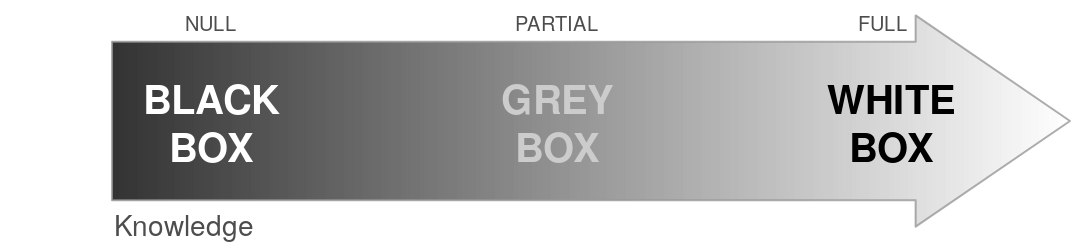
\includegraphics[width=.7\linewidth]{figures/pentest-types}
  \caption{Types of penetration test in function of the prior degree of knowledge}
  \label{fig:pentest-types}
\end{figure}

\subsection{Blackbox}

A black box is the representation of a system taking inputs and giving outputs, with no consideration of its internal functioning. This working is either inaccessible (simply not available or lost), or deliberately omitted (in order to simulate the conditions in which a real attacker would operate).

In the \textit{Blackbox} context, the pentester really puts himself in the shoes of an external attacker and starts his penetration test with as little information as possible on his target (his target then being the company having requested the assessment). Indeed, when the tester begins his attack, he does not have (or rarely) the complete map of the \acrshort{is}, the list of servers with their IP, and so forth. The \textit{Blackbox} context aims to find and demonstrate the presence of an actionable plan by an external person to take control of the \acrshort{is} or get hold of certain information.

Reasons for black box penetration testing :

\begin{itemize} \vspace{-.2cm}
  \item[\checkmark] Simulates the majority of potential attacks facing your organization
  \item[\checkmark] Helps to identify where your systems are weakest
  \item[\checkmark] Provides an objective, outsider’s view of your systems
\end{itemize}

\subsection{Whitebox}

In systems theory, a white box, is a module of a system that can be expected to work internally because we know the operating characteristics of all elements that compose it. In other words, a white box is a module that has as few black boxes as possible.

In this case, the pentester works in close collaboration with the DSI, the RSSI and the technical team of the information system. The goal is to obtain 100\% information on the information system and to support the CIO in the detection of vulnerability. One of the advantages of the White Box mode is that it is then possible to detect security flaws in a wider way and that the Black Box mode would not have made it possible to detect, for example if the pentester had not reached a certain stage of the intrusion. In addition, the White Box mode is more easily integrated into the \acrshort{is} lifecycle, sometimes at each stage of its evolution.

Reasons for white box penetration testing:
\begin{itemize} \vspace{-.2cm}
  \item[\checkmark] Efficient use of ethical hacker’s time
  \item[\checkmark] Provides “full disclosure” insights
  \item[\checkmark] Allows for objective scrutiny of internal systems
\end{itemize}

\subsection{Greybox}

An engagement that allows a higher level of access and increased internal knowledge falls into the category of gray-box testing. Comparatively, a black-box tester begins the engagement from a strict external viewpoint attempting to get in, while the gray-box tester has already been granted some internal access and knowledge that may come in the form of lower-level credentials, application logic flow charts, or network infrastructure maps. Gray-box testing can simulate an attacker that has already penetrated the perimeter and has some form of internal access to the network.

By providing some form of background to the security consultants undertaking the assessment, it helps to create a more efficient and streamlined approach. This saves on the time (and money) spent on the reconnaissance phase, allowing the consultants to focus their efforts on exploiting potential vulnerabilities in higher-risk systems rather than attempting to discover where these systems may be found.

Reasons for grey box penetration testing :
\begin{itemize} \vspace{-.2cm}
  \item[\checkmark] Focus the attention on more highly-valuable areas within the network
  \item[\checkmark] Increases the attack coverage and efficiency
  \item[\checkmark] Cost effective
\end{itemize}

\begin{info} \hyphenation{}
The point here is that the type of testing we will achieve will depend on the target, as only a few information or even none could be available. We will see that some models of target and their related manufacturers are not always very transparent, then forcing the test to be limited to blackbox.
\end{info}

\section{Methodologies \& Techniques}

This section presents some methodologies and techniques that will be used in the remainder of this work.

\subsection{\acrlong{ptes}}

After having introduced what is a pentest, let us look at a popular methodology for organizing a pentest.

\begin{question}
\textbf{But why do penetration testers need to follow a methodology ?}
\begin{itemize}
  \item The security world is changing fast, techniques and technologies are constantly changing, vulnerabilities are discovered on a daily basis. Faced with this, a bit of \textbf{structure} is needed. The methodologies allow to provide a fixed framework on the progress of a penetration test.
  \item Faced with an \acrshort{is} or many, a pentester has to look into each system, service, port or IP which can hide a vulnerability, see a path all traced until the takeover of the system. This multiplied by the very large amount of testing to be done depending on the service or technology used, makes it is easy to get lost. A framed and fixed methodology then makes it possible to follow a \textbf{canvas} and thus to organize the penetration test so that it is as \textbf{complete} as possible and \textbf{repeatable}.
  \item In the professional environment, \textbf{team working} is essential. This is also the purpose of common methodologies, norms and standards. A methodology known by several pentesters will facilitate and make more efficient the work within the team. Also, the report generated and the documentation will be made following a known frame : that of the methodology used.
\end{itemize}
\end{question}

First and foremost, a methodology will make it possible to not forget anything during the penetration test and to make sure that it is as complete as possible. During said pentest, the methodology acts as a way to follow, facilitating the organization of the pentester.

\paragraph{\acrfull{ptes} \cite{ptes}} Let's take a look at this popular methodogy that is often used by most pentesters. Mostly, this methodology is used as a basis in the pentest teams who customize them with their own methods, tools and techniques, which is what will make the difference between one team of pentest and another. The experience of the field is then added to the theory of the methodology. It should also be noted that each pentest follows a path of its own according to the \acrshort{is} to be tested. This methodology follows the steps as depicted in \ref{fig:ptes-process} and explained hereafter.

\begin{figure}[H]
  \centering
  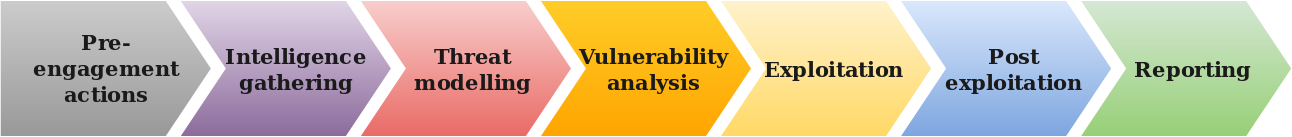
\includegraphics[width=\linewidth]{ptes-process}
  \caption{The 7 steps of \acrshort{ptes}}
  \label{fig:ptes-process}
\end{figure}

\begin{enumerate}
  \item \textbf{Pre-engagement Interactions} : Obviously, each intrusion test starts with a negotiation, an understanding of customer needs and finally a contractualization that puts all of this into paper form. The establishment of the contract is an opportunity for the company requesting the security test to specify several things concerning the scope of the intrusion test to be performed. In terms of time (days, weeks, months), in terms of technologies, in geographical terms (range of IP to test and not to test for example). Also, this is an opportunity to specify the type of test to be provided: can testers set up DoS attack phases ? Will they have to go to the end of the operation even if they have to open sensitive documents ? The contract also aims to establish a legal link and a protection for the pentester that could fall on sensitive documents, but also to negotiate and inform the companies collaborating with the customer (ISP, host, business application, etc.).
  \item \textbf{Intelligence Gathering} : The second step is that of "Intelligence Gathering" or "Information Gathering". Understandably the collection of information. Here, the pentester will try to list as much information about the SI tested, and this via several methods. The goal is therefore to map the attack surface from the starting position, to obtain information on the services, servers and active elements used, as well as their version and security systems in place (VPN, Firewall, Anti-Ddos, DMZ, etc.). The Intelligence Gathering part can be done passively (without direct interaction with the \acrshort{is} of the target) and / or actively (by going to communicate with the targeted servers). This also includes the concepts of OSINT (Open Source Intelligence) and HUMINT (Human Intelligence, understand social engineering).
  \item \textbf{Threat Modeling} : The third step is the Threat Modeling, in which the pentester is going to look for a list of threats for the company. What can the company have to deal with ? He will try to evaluate what is critical for the company (e.g. its manufacturing secret), to establish the potential impact of the loss of this secret and then see what vulnerabilities can lead to a loss of manufacturing secrecy. Also, one can go through an analysis phase in terms of security of competitors / similar companies. Have they been compromised recently ? What was the impact of the attack ? An analysis of the company's process and its human assets can also be performed as well as an analysis of the \acrshort{is}: is there an encryption mechanism for salespeople communicating with the inside of the \acrshort{is} on the business application ? Is a VPN in place for the remote administration of the \acrshort{is} ? The model should be clearly documented, and be delivered as part of the final report as the findings in the report will reference the threat model in order to create a more accurate relevance and risk score that is specific to the organization (rather than a generic technical one).
  \item \textbf{Vulnerability Analysis} : The information collected previously will be used to analyze the systems, staff and processes in place to search for exploitable vulnerabilities. Thus, it goes through a manual and / or automatic search process of vulnerabilities. The objective here is to draw up a list of what could be exploitable and build a "tree of attack", i.e. a continuation of attack that can lead to the discovery of other vulnerabilities, tracing a path towards the takeover of the \acrshort{is} or the possibility of establishing acts of espionage or sabotage. This phase is systematically based on research on the bases of public exploits, verification of the patches of the scanned systems and the use of scans tools (Ex: Nessus, OpenVAS, Nmap, etc.). If the vulnerability analysis phase was properly completed, a high value target list should have been complied. Ultimately the attack vector should take into consideration the success probability and highest impact on the organization.
  \item \textbf{Exploitation} : The fifth stage is often the most awaited of the pentesters, it is the moment to go to the attack: the exploitation. Here, he will try to test the vulnerabilities found in the previous phases and to advance in the intrusion of the information system. He will also try to test the barriers and security systems in place (evasion of an IDS, bypassing a security, bypass authentication). This will be followed by a validation process of the potential vulnerabilities found. It is important here to find ways to exploit vulnerabilities and also security systems. If the pentester advances in the SI, it may have to go back to step 4 in order to perform a new vulnerability analysis in the new zone (let's say if it manages to switch from the DMZ to the LAN). Note that in the pre-engagement interaction phase with the customer, a clear definition of the overall objectives of the penetration test should have been communicated. In the case of the exploitation phase, the biggest challenge is identifying the least path of resistance into the organization without detection and having the most impact on the organizations ability to generate revenue. By performing the prior phases properly, a clear understanding of how the organization functions and makes money should be relatively understood. From the exploitation phase and into the post-exploitation phase, the attack vectors should rely solely on the mission of circumventing security controls in order to represent how the organization can suffer substantial losses through a targeted attack against the organization.
  \item \textbf{Post Exploitation} : The purpose of the Post-Exploitation phase is to determine the value of the machine compromised and to maintain control of the machine for later use. This step has several interesting phases, like a real attacker, the pentester will have to erase his tracks so that these actions are as discreet as possible (clearing logs for example). Also, it will have to seek to establish a sustainable way in the information system by inserting backdoors, by creating a VPN account or by installing a malware / rootkit. The post-exploitation phase is also the last technical phase of the intrusion test, so it is time to target the information to be stolen (also referred as “Pillaging”), the interesting people of the company (trapping a high placed target for example). The idea here is to really show what mischief an attacker could accomplish: espionage, sabotage, exfiltration of data, deployment of a botnet, decommissioning part of the \acrshort{is}, etc.
  \item \textbf{Reporting} : The Pentest approach described in the PTES ends with the reporting phase, and this is the most important phase because it consists in exposing the progress of the intrusion test and its fruits to the client. Reporting will be both technical and non-technical. The pentester will then detail the information retrieved during the Intelligence Gathering phase, expose the vulnerabilities listed and exploited and describe the misdeeds that have / could have been perpetrated in the Post-Exploitation phase. This phase is often oral but is always accompanied by a written deliverable containing all this information. Finally, the pentest team is often called upon to draw up a "Remediation Roadmap", i.e. a list of countermeasures, corrections and protections to be put in place so that the company has tracks to start on following the securing of his \acrshort{is}.
\end{enumerate}

\subsection{Wireless penetration testing}


\subsection{Reverse engineering}


\subsection{Hardware hacking}


\begin{info}
For this work, we essentially apply the penetration testing methodology \acrshort{ptes} to wireless devices, using reverse engineering and hardware hacking to complement the assessment with in depth target understanding.
\end{info}


\section{Tools \& Resources}

In the past, hacking was difficult and required a lot of manual tinkering. Today, hackers have complete suites of automated test tools and processing capabilities that allow them to conduct much more sophisticated attacks, on much larger scales and much faster. In order to end framing the background, various existing security solutions are presented in order to get an overview of what could be usable in the implementation of a penetration test. The remaining of this section presents useful and popular tools distinguished by categories, relevant to penetration testing but not necessarily in our scope. For each tool, it is mentioned if it was used in this project or not.

\subsection{Pentesting platforms}

Two Linux distributions seem to be among the leaders regarding penetration testing ; Kali Linux \cite{kali-linux} and Parrot OS \cite{parrot-os}.

\begin{solutiondata}{kali}
\begin{itemize}[labelsep=1cm]
  \item [\textbf{Type}] Operating System
  \item [\textbf{Purpose}] Reconnaissance, vulnerability analysis, wireless attacks, web application attacks, sniffing and spoofing, reverse engineering, digital forensics, exploit creation, ...
  \item [\textbf{Pros}] Open-source \newline Community supported \newline Various command-line tools
  \item [\textbf{Used}] Yes
\end{itemize}
\end{solutiondata}

{\hyphenation{currently}
\textbf{Kali Linux} \cite{kali-linux} is a Debian-based distribution created by Offensive Security \cite{offensive-security} (another reference in security trainings and certifications) with advanced penetration testing features and tools. This is currently one of the most complete and powerful existing pentesting distributions. It also makes available various command-line tools that are appropriate for scripting and automation. A complete list of the available tools can be consulted at \cite{kali-linux-tools}. One can point out the Metasploit framework \cite{metasploit} as the most interesting and sophisticated tool to perform penetration tests and Volatility \cite{volatility} for digital forensics (essentially the analysis of memory dumps).}

\begin{solutiondata}{parrot}
\begin{itemize}[labelsep=1cm]
  \item [\textbf{Type}] Operating System
  \item [\textbf{Purpose}] Reconnaissance, vulnerability analysis, wireless attacks, web application attacks, sniffing and spoofing, reverse engineering, digital forensics, exploit creation, ...
  \item [\textbf{Pros}] Open-source \newline Lightweight \newline Various command-line tools
  \item [\textbf{Used}] No
\end{itemize}
\end{solutiondata}

\textbf{Parrot OS} \cite{parrot-os} is a free and open source GNU/Linux distribution based on Debian Testing designed for security experts, developers and privacy aware people. Originally developed as part of Frozenbox, the effort has grown to include a community of open source developers, professional security experts, advocates of digital rights, and Linux enthusiasts from all around the globe. It is intended to provide a suite of penetration testing tools to be used for attack mitigation, security research, forensics, and vulnerability assessment.

\subsection{Intelligence Gathering}

As previously evoked, the reconnaissance is the very first of the phases, and it is the one where the pentester will collect the maximum of data on its target before moving on to the following phases. There are a lot of different tools available to the attacker, here are presented a few of the most representative.

\begin{solutiondata}{google}
\begin{itemize}[labelsep=1cm]
  \item [\textbf{Type}] Search Engine
  \item [\textbf{Purpose}] Advanced search on Internet
  \item [\textbf{Pros}] Free \newline Easy to use \newline Finds information that is not readily available on a website
  \item [\textbf{Used}] Yes
\end{itemize}
\end{solutiondata}

\textbf{Google Hacking} \cite{google-hacking} is a technique that relies on the search power of the famous search engine to find accurate information that can help navigate a security breach. To use it, one has to use the Google Dork, they are specific search operators that allow to find accurate data, unlike every day searches, one types keywords in the search bar that can correspond to a text, a title, an image, a meta tag, an alternative text of an image and many others.

\begin{solutiondata}{shodan}
\begin{itemize}[labelsep=1cm]
  \item [\textbf{Type}] Search Engine
  \item [\textbf{Purpose}] Find vulnerable devices
  \item [\textbf{Pros}] Easy to use \newline Indexes all the things connected to the internet
  \item [\textbf{Used}] No
\end{itemize}
\end{solutiondata}

\textbf{Shodan} \cite{shodan} is a website specialized in finding objects connected to the Internet, and therefore having a visible IP address on the network. It allows to find a variety of web servers, routers and many devices such as printers or cameras. Such a request is processed with a simple analysis of the HTTP header returned by the device or server. It is then possible to retrieve lists of specific elements. For each result, it finds the IP address of the server as well as other types of sensitive but accessible information.

\begin{solutiondata}{maltego}
\begin{itemize}[labelsep=1cm]
  \item [\textbf{Type}] Data Mining tool
  \item [\textbf{Purpose}] Providing a library of transforms for discovery of data from open sources, and visualizing that information in a graph format, suitable for link analysis and data mining
  \item [\textbf{Pros}] Highly customizable \newline Graph export options \newline Runs on Windows, Mac and Linux
  \item [\textbf{Used}] No
\end{itemize}
\end{solutiondata}

\textbf{Maltego} \cite{maltego} can be used to determine the relationships between people, websites, documents and files... Connections between these pieces of information are found using open source intelligence (OSINT) techniques by querying sources such as DNS records, Whois records, search engines, social networks, various online APIs and extracting meta data. Maltego provides results in a wide range of graphical layouts that allow for clustering of information which makes seeing relationships instant and accurate – this makes it possible to see hidden connections even if they are three or four degrees of separation apart.

\subsection{Vulnerability Analysis}

New vulnerabilities are emerging every day, within networks, applications, databases. A vulnerability scanner is therefore a computer program designed to assess them for known weaknesses. They are utilized in the identification and detection of vulnerabilities arising from mis-configurations or flawed programming within a network-based asset such as a firewall, router, web server, application server, etc. Modern vulnerability scanners allow for both authenticated and unauthenticated scans. Once again, let’s have a look at some of the most popular ones.

\begin{solutiondata}{nmap}
\begin{itemize}[labelsep=1cm]
  \item [\textbf{Type}] Security Scanner, Port Scanner, Network Exploration Tool
  \item [\textbf{Purpose}] Identifying what devices are running on a network, discovering hosts that are available and the services they offer, finding open ports and detecting security risks
  \item [\textbf{Pros}] Free \newline Well documented \newline Includes many port scanning mechanisms
  \item [\textbf{Used}] Yes
\end{itemize}
\end{solutiondata}

\textbf{Nmap} \cite{nmap} ("Network Mapper") is a free and open source utility for network discovery and security auditing. Nmap uses raw IP packets in novel ways to determine what hosts are available on the network, what services (application name and version) those hosts are offering, what operating systems (and OS versions) they are running, what type of packet filters/firewalls are in use, and dozens of other characteristics. It was designed to rapidly scan large networks, but works fine against single hosts.

\begin{solutiondata}{wireshark}
\begin{itemize}[labelsep=1cm]
  \item [\textbf{Type}] Packet Analyzer
  \item [\textbf{Purpose}] Enables live data reading and analysis for a wide range of network protocols
  \item [\textbf{Pros}] Open Source \newline Display filters are used to filter and organize the data display \newline New protocols can be scrutinized by creating plug-ins
  \item [\textbf{Used}] Yes
\end{itemize}
\end{solutiondata}

\textbf{Wireshark} \cite{wireshark} intercepts traffic and converts that binary traffic into human-readable format. This makes it easy to identify what traffic is crossing a network, how much of it, how frequently, how much latency there is between certain hops, and so forth. While Wireshark supports more than two thousand network protocols, many of them esoteric, uncommon, or old, the modern security professional will find analyzing IP packets to be of most immediate usefulness. The majority of the packets on your network are likely to be TCP, UDP, and ICMP.

\begin{solutiondata}{nessus}
\begin{itemize}[labelsep=1cm]
  \item [\textbf{Type}] Vulnerability Scanner
  \item [\textbf{Purpose}] Identifying what devices are running on a network, discovering hosts that are available and the services they offer, finding open ports and detecting security risks
  \item [\textbf{Pros}] Highly customizable \newline Covers a wide range of technologies \newline Automated reports
  \item [\textbf{Cons}] Full version is expensive
  \item [\textbf{Used}] No
\end{itemize}
\end{solutiondata}

\textbf{Nessus} \cite{Nessus} is a proprietary vulnerability scanner developed by Tenable. Nessus detects live machines on a network, scans open ports, identifies active services, their version, and then attempts various attacks. He then points out the potential or proven weaknesses on the tested machines on a global report. Nessus scans cover a wide range of technologies including operating systems, network devices, hypervisors, databases, web servers, and critical infrastructure. Since version 3, it is licensed, but still free for personal use. Version 2 is maintained. There is also a fork of Nessus 2 still under GPL license called OpenVAS.

\subsection{Exploitation}

With a map of all possible vulnerabilities and entry points, the pentester begins to test the exploits found within your network, applications, and data. The goal is for the ethical hacker is to see exactly how far they can get into your environment, identify high-value targets, and avoid any detection. These actions are once again made easier with the help of multiple tools, some of which are discussed below.

\begin{solutiondata}{metasploit}
\begin{itemize}[labelsep=1cm]
  \item [\textbf{Type}] Penetration Testing Framework
  \item [\textbf{Purpose}] Tool for developing and executing exploit code against a remote target machine
  \item [\textbf{Pros}] Rather intuitive \newline Currently has over 1600 exploits \newline Large user community
  \item [\textbf{Used}] No
\end{itemize}
\end{solutiondata}

\textbf{The Metasploit Framework} \cite{metasploit} is a Ruby-based, modular penetration testing platform that enables to write, test, and execute exploit code. The Metasploit Framework contains a suite of tools that can be used to test security vulnerabilities, enumerate networks, execute attacks, and evade detection. At its core, the Metasploit Framework is a collection of commonly used tools that provide a complete environment for penetration testing and exploit development. More specifically, the MSFconsole provides a command line interface to access and work with the Metasploit Framework. The console lets you do things like scan targets, exploit vulnerabilities, and collect data.

\begin{solutiondata}{john}
\begin{itemize}[labelsep=1cm]
  \item [\textbf{Type}] Offline Password Cracker
  \item [\textbf{Purpose}] Test the security of a password, crack password hashes
  \item [\textbf{Pros}] Open source \newline Extensible (for new crackable hash types) \newline Can leverage graphical card's GPU power for a better performance
  \item [\textbf{Used}] Yes
\end{itemize}
\end{solutiondata}

\textbf{John the Ripper} \cite{john} is a free software for breaking a password, used in particular to test the security of a password. First developed to run under UNIX-derived systems, the program now operates under fifty different platforms, such as BeOS, BSD and its derivatives, DOS, Linux, OpenVMS, Win32. John is one of the most popular password cracking software because it includes the autodetection of hash functions used to store passwords, the implementation of a large number of cracking algorithms, by the fact that it is very easily modifiable, and also that it is possible to resume an attack after a pause.

\begin{solutiondata}{hydra}
\begin{itemize}[labelsep=1cm]
  \item [\textbf{Type}] Online Password Cracker
  \item [\textbf{Purpose}] Test the security of a password, crack passwords on live services
  \item [\textbf{Pros}] Open source \newline Supports a large set of different password hash types \newline Possible to restore a previous aborted/crashed session
  \item [\textbf{Used}] Yes
\end{itemize}
\end{solutiondata}

\textbf{Hydra} \cite{hydra} is a parallelized login cracker which supports numerous protocols to attack. It is very fast and flexible, and new modules are easy to add. Hydra is often John's accomplice. It can take over to break a password online, for example an SSH or FTP, IMAP, IRC, RDP and more. Just point Hydra to the service you want to hack, provide it a list of words, and launch it. Tools like Hydra point out that limiting the password rate and disconnecting users after several unsuccessful login attempts are effective defensive measures against attackers.

\begin{solutiondata}{burp}
\begin{itemize}[labelsep=1cm]
  \item [\textbf{Type}] Web Application Testing
  \item [\textbf{Purpose}] Identify vulnerabilities and verify attack vectors that are affecting web applications
  \item [\textbf{Pros}] Can be used to modify requests to the server, resend them, and observe the results \newline Reported vulnerabilities contain detailed custom advisories
  \item [\textbf{Used}] No
\end{itemize}
\end{solutiondata}

\textbf{Burp Suite} \cite{burp} is a Java based Web Penetration Testing framework. It has become an industry standard suite of tools used by information security professionals. Burp Suite helps you identify vulnerabilities and verify attack vectors that are affecting web applications. In its simplest form, Burp Suite can be classified as an Interception Proxy. While browsing their target application, a penetration tester can configure his internet browser to route traffic through the Burp Suite proxy server. Burp Suite then acts as a (sort of) “Man in The Middle” by capturing and analyzing each request to and from the target web application. Penetration testers can pause, manipulate and replay individual HTTP requests in order to analyze potential parameters or injection points. Injection points can be specified for manual as well as automated fuzzing attacks to discover potentially unintended application behaviors, crashes and error messages.

\begin{solutiondata}{aircrack-ng}
\begin{itemize}[labelsep=1cm]
  \item [\textbf{Type}] WiFi attacks toolkit
  \item [\textbf{Purpose}] Packet sniffing and injection, WEP encryption key recovery
  \item [\textbf{Pros}] Focuses on different areas of WiFi security: monitoring, attacking, testing and cracking \newline All tools are command line which allows for heavy scripting
  \item [\textbf{Used}] Yes
\end{itemize}
\end{solutiondata}

\textbf{Aircrack-ng} \cite{aircrack-ng} is a complete suite of tools to assess WiFi network security. It focuses on different areas of WiFi security :
\begin{itemize}
  \item Monitoring : Packet capture and export of data to text files for further processing by third party tools
  \item Attacking : Replay attacks, deauthentication, fake access points and others via packet injection
  \item Testing : Checking WiFi cards and driver capabilities (capture and injection)
  \item Cracking : WEP and WPA PSK (WPA 1 and 2)
\end{itemize}

\subsection{Reverse engineering}

\textbf{ILSpy}

\textbf{Hopper Disassembler}


\end{chaptercover}
